\section{Approach overview}\label{sect:overview}

\begin{figure*}[t!]
  \centering
  \hspace*{-0.35em}
  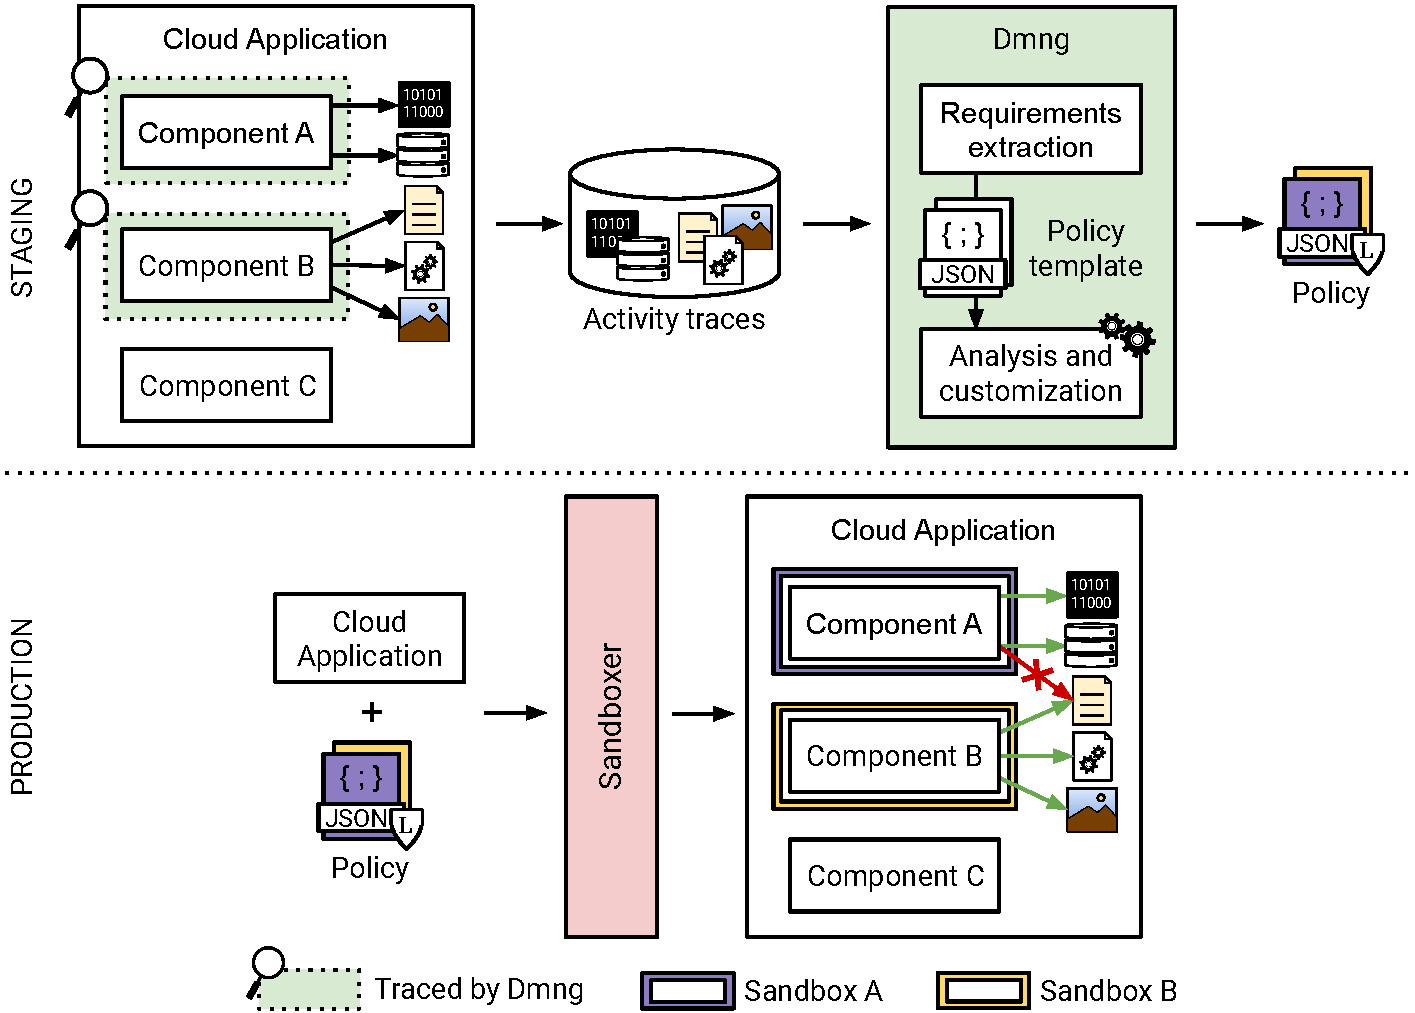
\includegraphics[width=1.01\linewidth]{chapters/dmng/fig/staging-prod.pdf}
  \caption[Overview of our approach]{Approach overview: 1)~\dmng uses
    probes to trace the application components A and B, 2)~activity
    traces are saved into a SQLite DB, 3)~requirements are extracted
    from the traces and used to build security policies, finally
    4)~policies are leveraged by the sandboxer to secure the
    application in production}
  \label{fig:overview}
\end{figure*}

Frequently, developers start building cloud applications from base
container images, which are subsequently customized and extended with
third-party software (e.g., web frameworks, database drivers, etc.).
Once the application has been developed, it is released to the staging
area, a replica of the production environment, not accessible from the
outside, where developers and cloud architects can test new features
so to detect design flaws and prevent unexpected errors to hit the
production environment.  The similarity to the production area makes
it the best candidate to generate accurate least privilege policies to
restrict the permissions available to the application.

To operate as intended, each application component requires access to
system resources like programs, scripts, dynamic libraries, shared
memory, and files. We simply call these resources {\em requirements}.
In order to collect them, we provide an intuitive open source tool
called \dmng that performs service instrumentation as shown in
Figure~\ref{fig:overview}.  In detail, the tool leverages ptrace and
eBPF to setup and activate temporary probes that register the actions
performed by an application component, making it possible to track
file-opening requests, reading and writing of data, use of shared
memory and execution of native code via subprocesses and shared
libraries. All these requests are automatically registered into a
database and subsequently used to generate policy templates. Together
with the file system path, each requirement is associated with
permissions. Compatibly with Unix-like systems, three permissions are
available: {\em read}, {\em write}, and {\em exec}. The policy
templates generated by \dmng can then be interactively modified by the
developer with the addition, modification or removal of policy
rules. After the changes are committed, the policy is serialized into
a JSON file and it is ready to be used to sandbox the application.

Sandboxing can be introduced with several technologies and frameworks;
given that we aim to restrict file system resources, we provide a
sandboxing utility based on Landlock that parses the set of
requirements needed by the application (i.e., path and permission
pairs) from the JSON policy file generated by \dmng, and it restricts
the permissions accordingly. We selected Landlock due to its
outstanding performance and stackability property.  Indeed, the use of
Landlock allows us to be compatible with systems that already rely on
other LSMs (e.g., AppArmor, SELinux).  We highlight that, whenever two
or more LSMs are available on the host, a single denial prevents the
access to a resource (i.e., deny takes precedence).

After the cloud application has been deployed to the production
environment it is important to ensure that services are running as
expected, there are no anomalies, and proactive measures are taken to
identify potential threats. By default, access to any file system
resource not listed in the policy is blocked by Landlock. However,
there may be cases in which the developer would like to generate
reports on the set of requested resources by the application. To
enable this, \dmng allows to temporarily observe and record the
activity traces generated by any application component without changes
to the application itself nor its execution state. These checks are
not bypassable, which is a considerable advantage compared to
alternative techniques that either rely on LD\textunderscore PRELOAD
or perform instrumentation through code dependency injection.

The following sections are organized as
follows. Section~\ref{sect:cloud-instrum} details the technologies
used to support policy generation and implement
monitoring. Section~\ref{sect:policy} clarifies the structure of the
policy. Section~\ref{sect:sandbox} describes sandboxing through
Landlock. Lastly, Section~\ref{sect:exp} showcases the mitigation
capabilities and investigates the performance overhead.


%%% Local Variables:
%%% mode: latex
%%% TeX-master: "../main"
%%% End:
